\documentclass[tikz,border=3pt]{standalone}
\usepackage[utf8]{inputenc}
\usepackage{tikz}
\usetikzlibrary{decorations.pathmorphing,arrows.meta}

\begin{document}
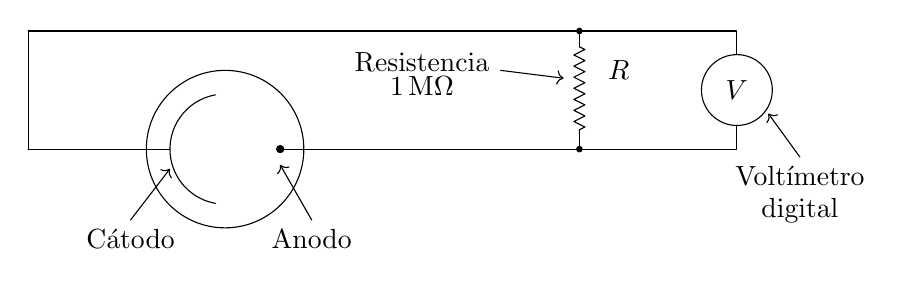
\begin{tikzpicture}[line cap=round,line join=round]

  %-------------------------
  % Circuito exterior
  %-------------------------
  \draw (-4,1.5) -- (3,1.5);      % parte superior
  \draw (-4,1.5) -- (-4,0);       % lado izquierdo
  \draw (-4,0) -- (-2.2,0);       % hasta el tubo
  \draw (-0.8,0) -- (0.8,0) -- (3,0); % desde ánodo hacia la derecha

  %-------------------------
  % Tubo fotoeléctrico
  %-------------------------
  % Circunferencia exterior
  \draw (-1.5,0) circle (1);

  % Cátodo: electrodo curvo interno
  % Ahora es un "C" abierto hacia la derecha, como en la figura original.
  \draw (-1.5,0) ++(100:0.7)
        arc[start angle=100,end angle=260,radius=0.7];

  % Ánodo: punto a la derecha
  \fill (-0.8,0) circle (1.5pt);

  % Etiquetas: cátodo
  \draw [->] (-2.7,-0.9) -- (-2.2,-0.25);
  \node[below] at (-2.7,-0.9) {C\'atodo};

  % Etiquetas: ánodo
  \draw [->]  (-0.4,-0.9) --  (-0.8,-0.2);
  \node[below] at (-0.4,-0.9) {Anodo};

  %-------------------------
  % Texto de la resistencia de 1 MΩ
  %-------------------------
  \node at (1,1.1) {Resistencia};
  \node at (1,0.8) {$1\,\mathrm{M}\Omega$};

  %-------------------------
  % Resistencia R en el lado derecho
  %-------------------------
  \fill (3,1.5) circle (1.2pt);
  \fill (3,0)   circle (1.2pt);

  \draw (3,1.5) -- (3,1.3);
  \draw (3,0.2) -- (3,0);

  \draw[decorate,decoration={zigzag,segment length=4pt,amplitude=2pt}]
       (3,1.3) -- (3,0.2);

  \node at (3.5,1.0) {$R$};
  \draw[->] (2,1.0) -- (2.8,0.9);

  %-------------------------
  % Voltímetro digital
  %-------------------------
  \draw (3,1.5) -- (5,1.5) -- (5,1.2);
  \draw (3,0)   -- (5,0)   -- (5,0.3);

  \draw (5,0.75) circle (0.45);
  \node at (5,0.75) {$V$};

  \draw [->] (5.8,-0.1) -- (5.4,0.45);
  \node[below] at (5.8,-0.1) {Volt\'imetro};
  \node[below] at (5.8,-0.5) {digital};

\end{tikzpicture}
\end{document}

